\documentclass[11pt,professionalfonts]{beamer}
\usefonttheme{serif}

\usepackage{presentation_packages}
\bibliography{library} % must be in the preamble when using biblatex package

\definecolor{mygray}{gray}{0.9}
\definecolor{RoyalBlue}{rgb}{0.25,0.41,0.88}
\def\Emph{\textcolor{RoyalBlue}}

\definecolor{tmp}{rgb}{0.804,0.941,1.0}
\setbeamercolor{numerical}{fg=black,bg=tmp}
\setbeamercolor{exact}{fg=black,bg=red}

\mode<presentation> 
{
  \usetheme{Warsaw}
  \usefonttheme{serif}
  \setbeamercovered{transparent}
}

\setbeamertemplate{footline}%{split theme}
{%
  \leavevmode%
  \hbox{\begin{beamercolorbox}[wd=.5\paperwidth,ht=2.5ex,dp=1.125ex,leftskip=.3cm,rightskip=.3cm plus1fill]{author in head/foot}%
    \usebeamerfont{author in head/foot}\insertshorttitle
  \end{beamercolorbox}%
  \begin{beamercolorbox}[wd=.5\paperwidth,ht=2.5ex,dp=1.125ex,leftskip=.3cm,rightskip=.3cm]{title in head/foot}
%    \usebeamerfont{title in head/foot}\mypaper\hfill \insertframenumber/\inserttotalframenumber
    \usebeamerfont{title in head/foot}\hfill \insertframenumber/\inserttotalframenumber
  \end{beamercolorbox}}%
  \vskip0pt%
} \setbeamercolor{box}{fg=black,bg=yellow}


\title[Lesson 02 - Installation]{\large \textbf{Installing Python}}

\author{\vspace*{-0.3cm}}

   
\institute{
  \footnotesize
  {\normalsize\bf{Shankar Kulumani}}\\
  \vspace*{0.2cm}
    \textbf{Flight Dynamics \& Control Lab}\\ \vspace*{0.5cm}
  \begin{figure} %figure%
        
\includegraphics[width=0.75\textwidth]{figures/gw_txh_2cs_pos.pdf}
    \end{figure}
}
\date{}

\begin{document}
%=======================================================%

\setcounter{framenumber}{-1}
\begin{frame} %-----------------------------%
  \titlepage
\end{frame}   %-----------------------------%

\section*{}
\subsection*{What is Python?}  
\begin{frame}{Get Scientific Python!}
\begin{columns}
\begin{column}{0.5\textwidth}
\begin{itemize}
    \item Python is a general language, but we care about the science!
    \item Use the \href{https://www.continuum.io/downloads}{Anaconda} distribution
    \item Includes everything we need 
\end{itemize}
\end{column}
\begin{column}{0.5\textwidth}
    \begin{figure}
        \centering
        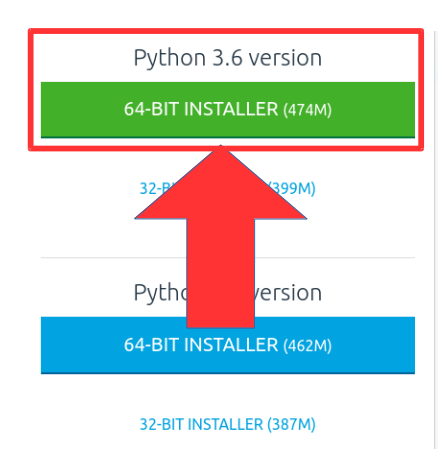
\includegraphics[width=\columnwidth,height=0.8\textheight,keepaspectratio]{figures/anaconda3.png}
        \caption{You want Python 3}
    \end{figure}
\end{column}
\end{columns}
\end{frame}

\begin{frame}{Using Python}
    \begin{itemize}
        \item Only need to use the ``command line'' and a text editor
            \begin{itemize}
                \item Win - \texttt{cmd}, OSX - \texttt{Terminal}, Linux
                \item Atom, Sublime, Notepad++
                    \begin{itemize}
                        \item Use 4 spaces instead of tabs
                    \end{itemize}
            \end{itemize}
    \end{itemize}
    \begin{figure}
        \centering
        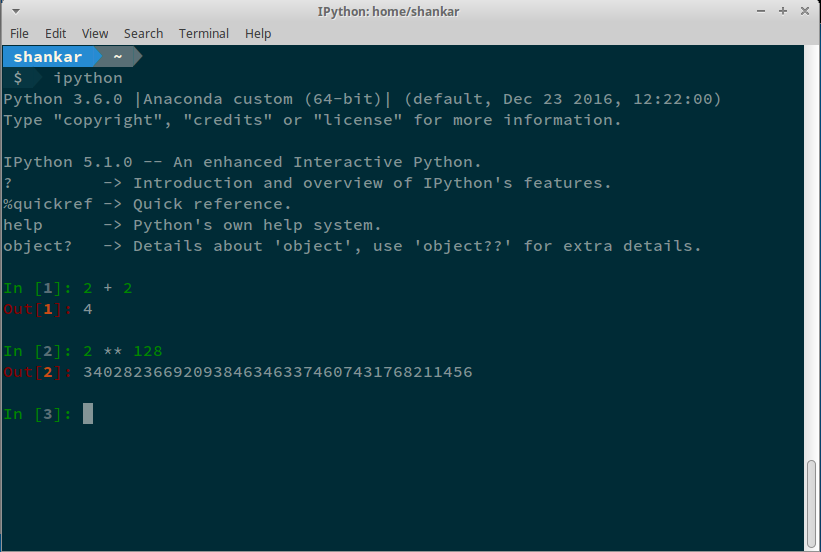
\includegraphics[width=\textwidth, height=0.6\textheight, keepaspectratio]{figures/starting_python.png}
    \end{figure}
\end{frame}

\begin{frame}{Real Programmers}
    \centering
    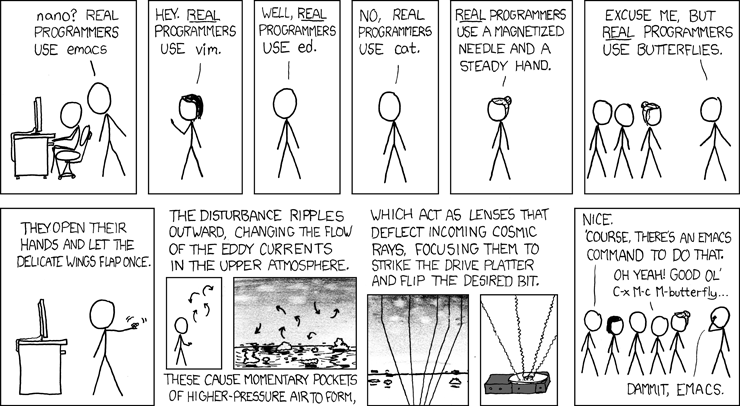
\includegraphics[width=\textwidth]{figures/real_programmers.png}
\end{frame}

\begin{frame}{History of Python}
    \begin{columns}
    \begin{column}{0.5\textwidth}
        \begin{itemize}
            \item \href{https://en.wikipedia.org/wiki/Guido_van_Rossum}{Guido van Rossum} started creating Python in 1989
        \end{itemize}
        \begin{block}{}
        Over six years ago, in December 1989, I was looking for a "hobby" programming project that would keep me occupied during the week around Christmas. \ldots I chose Python as a working title for the project, being in a slightly irreverent mood (and a big fan of Monty Python's Flying Circus).
        \end{block}
    \end{column}
    \begin{column}{0.5\textwidth}
        \begin{figure}
            \centering
            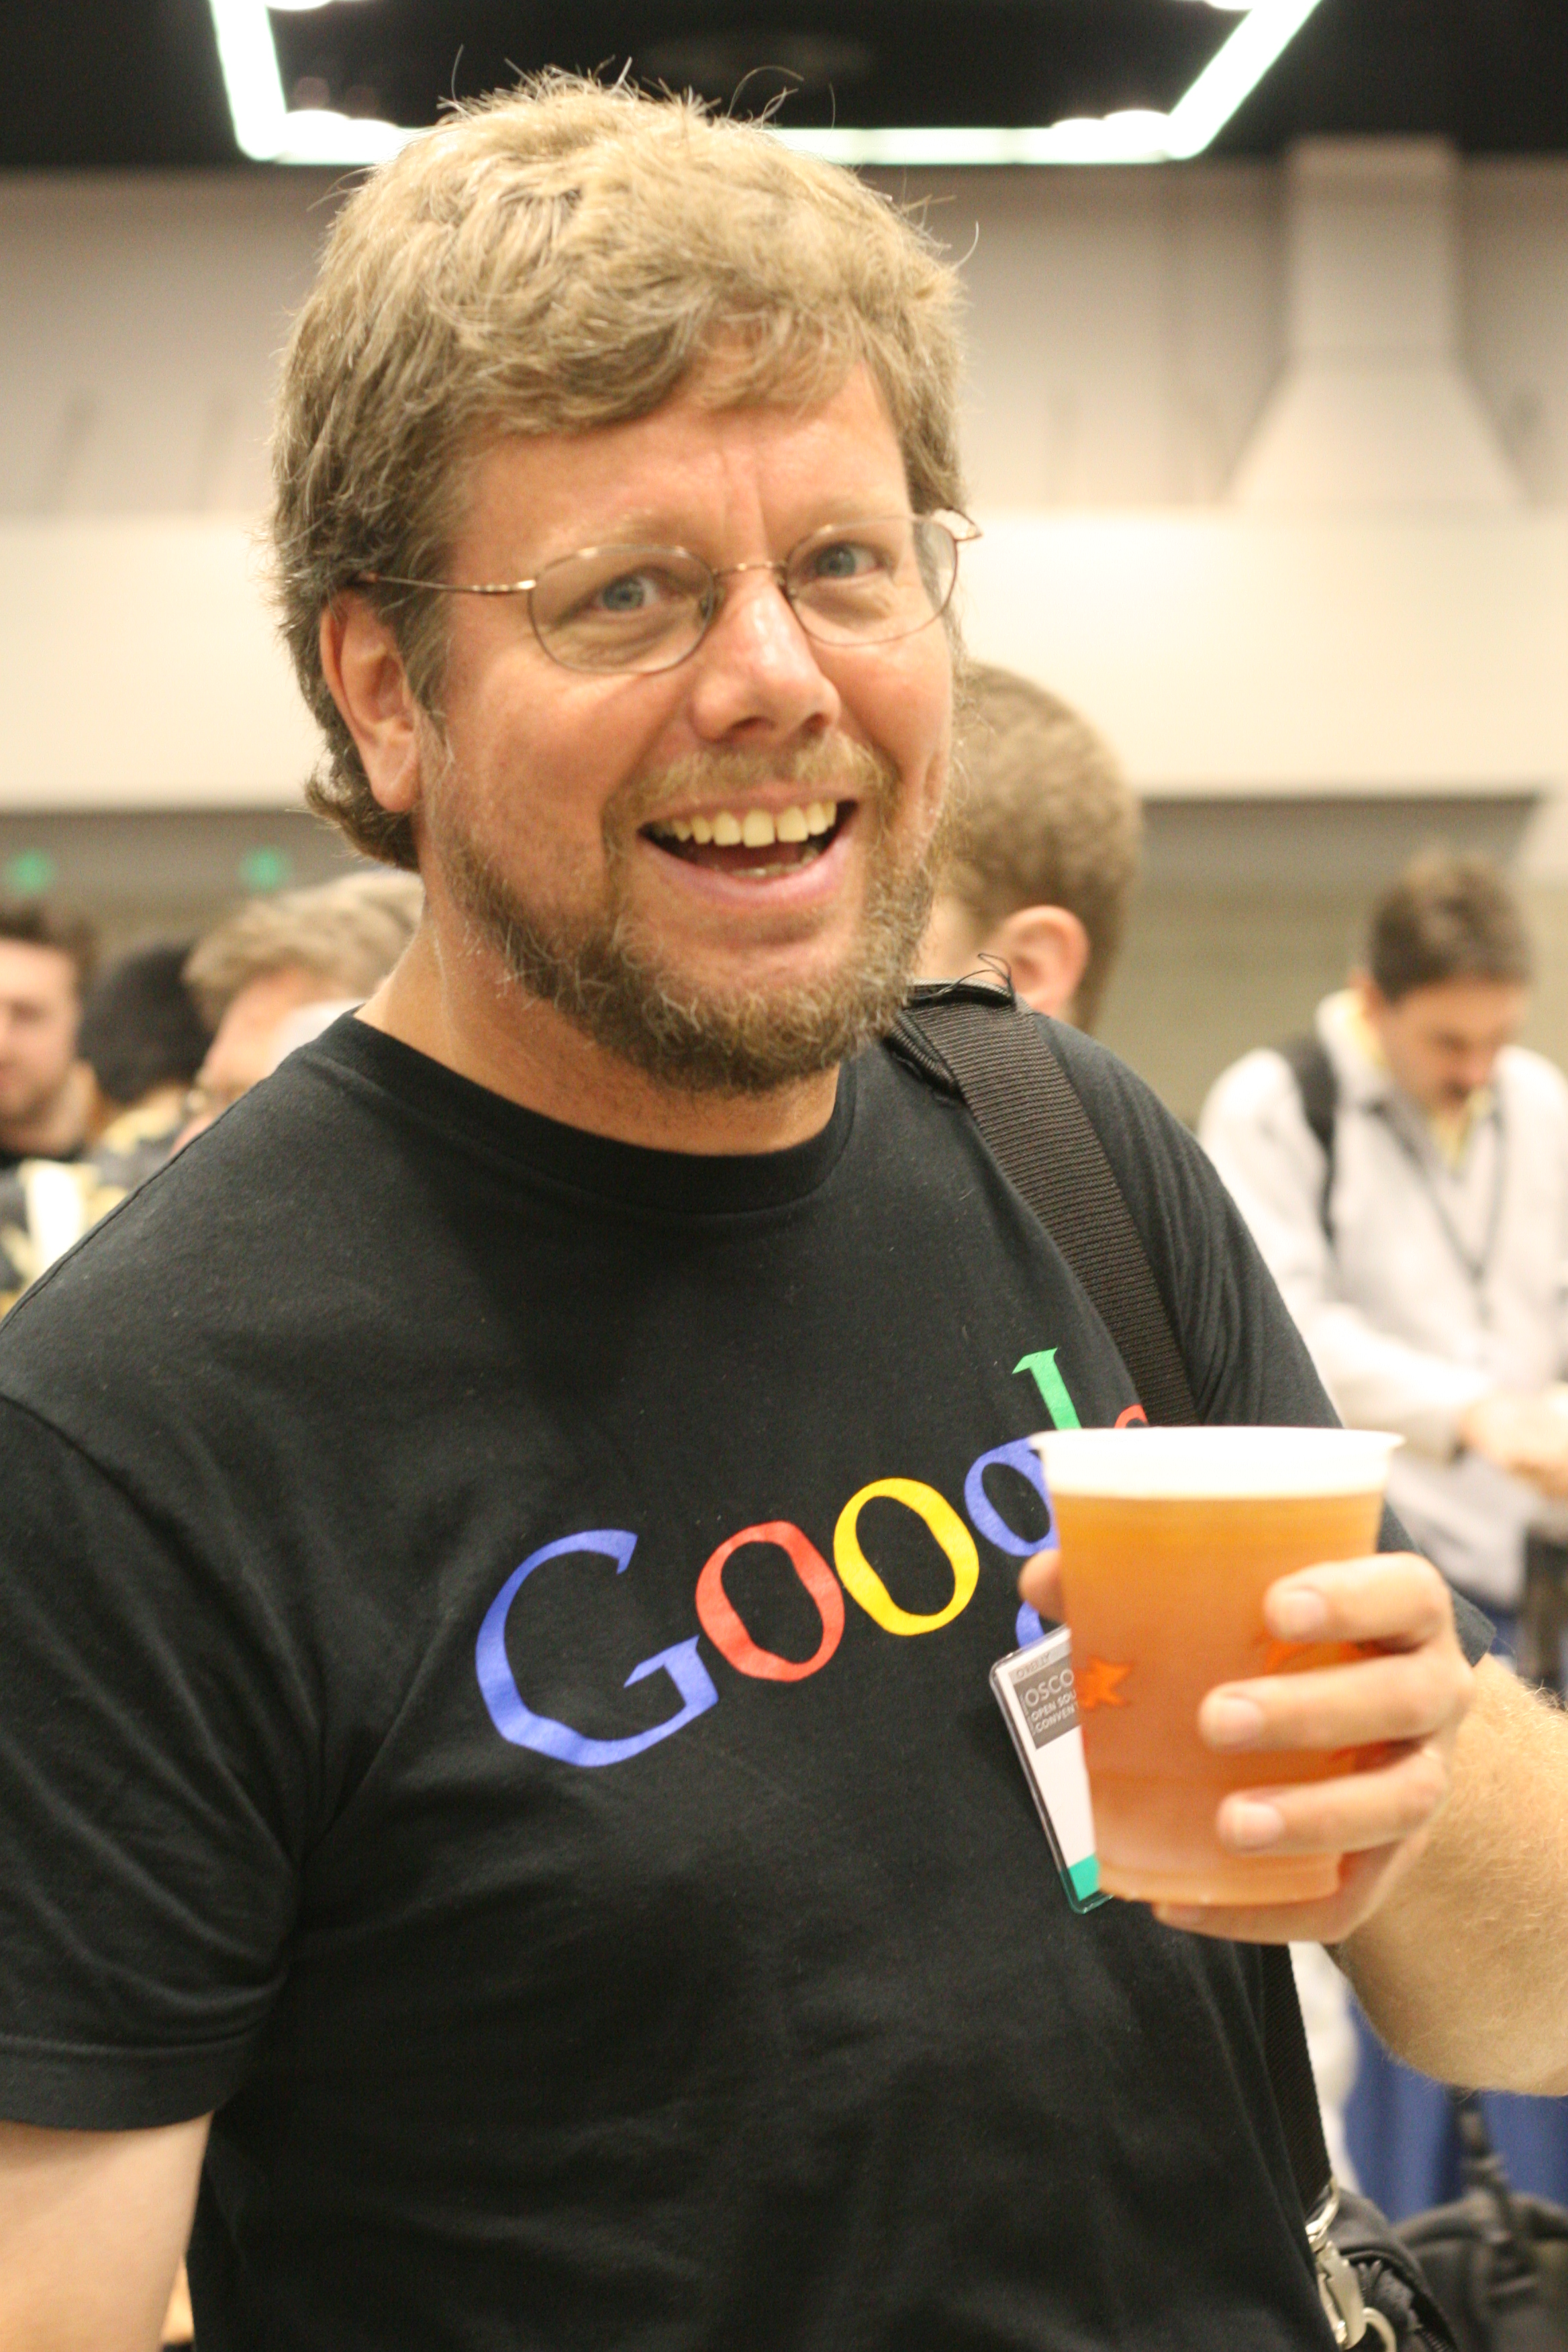
\includegraphics[keepaspectratio,height=0.8\textheight,width=\columnwidth]{Guido_van_Rossum_OSCON_2006}
            \caption{``Benevolent Dictator For Life''}
        \end{figure}
    \end{column}
    \end{columns}
\end{frame}

\begin{frame}{What is Python?}

Python is a modern, general-purpose, object-oriented, high-level language.

\begin{itemize}
    \item \emph{clean and simple language}: Easy to read and easy to learn syntax
    \item \emph{expressive language}: Fewer lines of code = fewer mistakes
    \item \emph{dynamically typed}: no need to define variable types or function arguments
    \item \emph{automatic memory management}: no need to allocate/deallocate memory
    \item \emph{interpreted}: No need to compile! Fast and easy
\end{itemize}

\end{frame}

\begin{frame}{No more compiling!}
    \centering
    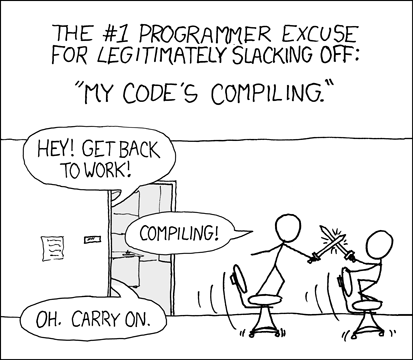
\includegraphics[height=0.8\textheight, keepaspectratio,width=\textwidth]{figures/compiling.png}
\end{frame}

\begin{frame}{Why Python?}
    \begin{columns}
    \begin{column}{0.5\textwidth}
    \begin{itemize}
        \item Free - free as in beer \Emph{AND} free as in speech
        \item General purpose - packages/modules for everything!
        \item Dynamic - no compiling
        \item Easy to read - enforces good structure!
        \item Open - everything is an object
    \end{itemize}
    \pause
    \begin{block}{}
        It's harder to read code than to write it!
    \end{block}
    \end{column}
    \begin{column}{0.5\textwidth}
        \begin{figure}
            \centering
            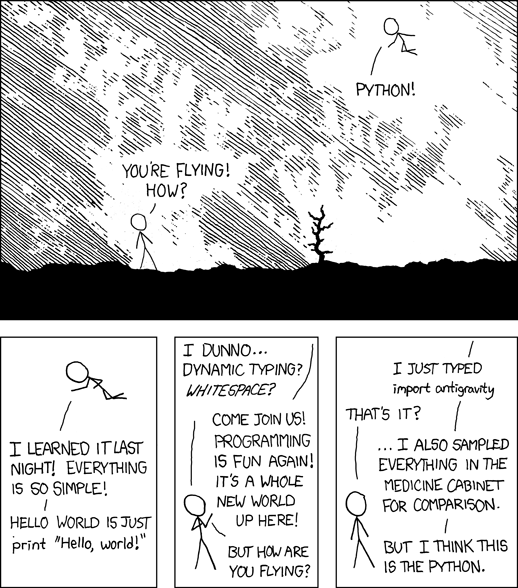
\includegraphics[width=\columnwidth,height=0.8\textheight,keepaspectratio]{figures/python.png}
        \end{figure}
    \end{column}
    \end{columns}
\end{frame}

\begin{frame}{Reading bad code}
    \centering
    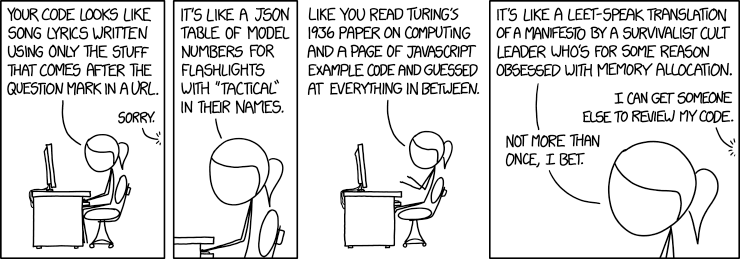
\includegraphics[width=\textwidth, height=\textheight,keepaspectratio]{figures/code_quality_3.png}
\end{frame}

\begin{frame}{Python vs. Matlab}
\begin{columns}[t]
\begin{column}{0.5\textwidth}
Disadvantages:
    \begin{itemize}
        \item Matlab is a commercial product - entire computing environment with code, IDE
        \item Matlab is expensive - Between \$49 - \$2150 per license! Extra for toolboxes
        \item Matlab is proprietary - Cannot inspect source code and restrictions on sharing 
        \item Matlab is closed - difficult to extend functionality 
    \end{itemize}
\end{column}
\pause
\begin{column}{0.5\textwidth}
    Advantages:
    \begin{itemize}
        \item Matlab handles arrays automatically and by design
        \item Lots of functionality - control design, linear algebra, optimization, ODEs etc.
        \item Real engineers (with funding) use it so students have to as well
        \item Simulink is still unmatched
        \item Powerful plotting capability
    \end{itemize}
\end{column}
\end{columns}
\pause
\begin{alertblock}{}
    \centering
    Python can offer all of the same functionality and some extra!
\end{alertblock}
\end{frame}

\begin{frame}{Python vs. Matlab}
    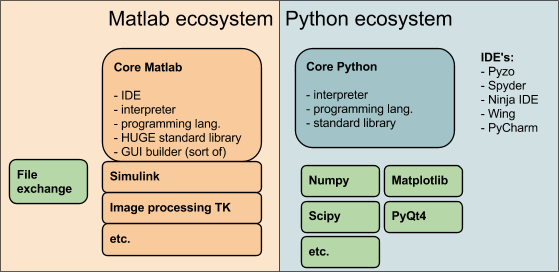
\includegraphics[width=\textwidth, height=\textheight, keepaspectratio]{figures/pythonvsmatlab.png}
\end{frame}

\begin{frame}{Learning Python 3}
    \begin{itemize}
        \item We have Python installed from Anaconda
        \item There are many, many free Python tutorials online
            \begin{itemize}
                \item \href{https://learnpythonthehardway.org/python3/}{Learn Python 3 the Hard Way}
                \item \href{https://docs.python.org/3/tutorial/index.html}{Python Tutorial}
                \item Go through these to learn the basics of Python!
            \end{itemize}
    \end{itemize}
\end{frame}
\end{document}

